% ========================================
% CHAPTER 3: RELATED WORK (WHAT WAS PREVIOUSLY DONE)
% ========================================
\chapter{Related Work}


% ========================================
% SECTION 3.1: ARCHITECTURAL APPROACHES FOR LONG CONTEXT MODELING
% ========================================
\section{Architectural Approaches for Long Context Modeling}

Long-context modeling must address the quadratic cost of vanilla self-attention \cite{vaswani_attention_2017} while preserving task-relevant dependencies over thousands of tokens.

A useful taxonomy distinguishes:
\begin{itemize}
    \item attention variants that alter the attention operator itself;
    \item explicit compression methods that reduce the input via retrieval or summarization;
    \item implicit compression methods that learn compact, decoder-friendly representations without exposing full inputs during inference.
\end{itemize}

We briefly review each group and summarize advantages and limitations.

\paragraph{Attention variants.}
Sparse and local/windowed patterns reduce pairwise interactions to achieve sub-quadratic cost.
Windowed attention restricts each token to a fixed neighborhood and optionally augments a small set of global tokens to propagate long-range information.
Longformer combines sliding windows with learnable global tokens for long documents \cite{beltagy_longformer_2020}.
Block- and mixed-sparsity patterns (e.g., banded + random) as in BigBird provide theoretical expressivity and empirical gains on long sequences \cite{zaheer_bigbird_2020}.
Sparse Transformers \cite{child_sparse_2019} introduced fixed sparse patterns for scalable generation.
Advantages include improved memory/computation and strong local modeling.
Disadvantages include potential failures to route cross-window interactions when global tokens or connectivity patterns are insufficient, and hardware inefficiencies for irregular sparsity.

Linear-time approximations further change the attention operator.
Kernelized attention (Transformers-as-RNNs) linearizes softmax attention for autoregressive decoding \cite{katharopoulos_transformers_2020}.
Linformer projects keys/values along sequence length to attain linear complexity \cite{wang_linformer_2020}.
These methods offer asymptotic gains and longer feasible contexts.
However, they can underperform full attention on tasks requiring precise long-range interactions or exact softmax geometry.
They also introduce approximation/projection hyperparameters that affect quality.

\paragraph{Explicit compression.}
Retrieval-augmented generation (RAG) or summarization-based pipelines reduce the effective input by selecting or rewriting content before decoding.
RAG retrieves top-$k$ passages from an external corpus and conditions generation on them.
This approach improves knowledge-intensive tasks while decoupling parametric and non-parametric knowledge \cite{lewis_rag_2020}.
Abstractive summarization pre-compresses long inputs into concise proxies (e.g., PEGASUS pretraining with gap-sentence objectives) \cite{zhang_pegasus_2020}.
Benefits include controllable compute and access to external knowledge.
Drawbacks include selection bias, retrieval latency, brittleness to retrieval errors, and potential loss of details critical for downstream reasoning.

\paragraph{Implicit compression.}
Here, the idea is to produce task-adapted representations (often embeddings) that a model uses during inference, rather than the input itself.
Examples include learned soft/prefix prompts for steering frozen decoders \cite{li_prefix_2021,lester_prompt_2021}.
Other examples include tokenized memories trained to preserve answer-relevant information.
Implicit methods maintain a tight interface to the model.
They can reduce latency and memory without external retrieval.
A key challenge of implicit compression is that, by condensing input into a compact intermediate representation, some information may inevitably be lost and cannot be recovered with perfect fidelity. 
This may limit the utility of compressed representations, especially when critical details are omitted during the compression process.

Taken together, attention variants trade exactness for structure or approximation.
Explicit compression trades completeness for selection.
\textbf{TODO: this is bullshit but make a change to section 3./ we like implicit so we found ICAE---} --- Implicit compression trades human readability for decoder-optimized compact interfaces.

% Insbesondere weisen wir auf den wunderbaren Artikel von \textcite{Edmonds:1965} und auf~\cite{GareyJohnson:1979} für weitere Hintergründe.


% ========================================
% SECTION 3.2: SOFT PROMPTING, CONTEXT DISTILLATION, AND CONTINUOUS-THOUGHT REPRESENTATIONS
% ========================================
\section{Soft Prompting, Context Distillation, and Continuous-Thought Representations}

Soft prompting is a method for conditioning large language models by learning continuous prompt vectors or prefix tokens rather than discrete text. 
These learned vectors are typically prepended to the model's input sequence and serve as a compact, trainable interface for adapting frozen decoders.
Classic methods in this category include prefix-tuning \cite{li_prefix_2021} and prompt tuning \cite{lester_prompt_2021}.
Both approaches involve optimizing a small set of continuous embeddings that steer the model toward desired behavior without full-scale model finetuning.
This parameter-efficient interface enables flexible adaptation and can be tuned for domain- or task-specific goals.
Because the prompt vectors are not constrained to map onto human-readable tokens, they can condense much more information than would be possible with standard textual prompts.

In practical, agentic settings the challenge of long or growing histories becomes acute (???).
%Models can distill the relevant information into a compact embedding or set of memory tokens.
%This reduces latency and memory overhead, as only condensed facts are passed forward during multi-step interactions.
%Examples of this pattern include ReAct-style prompting, which accumulates observations and actions over iterative reasoning steps \cite{yao_react_2022}, and Toolformer, which learns to use tools with self-supervised trajectories and requires summarizing complex action histories \cite{schick_toolformer_2023}.
%A scientific motivation for context distillation and soft prompting is that the resulting compression can be optimized directly for downstream utility, such as task success, rather than mere faithfulness to the original text.
%By learning what to keep and what to discard, these methods can mitigate biases and error propagation that affect explicit retrieval or summarization.

\textbf{CoConut} (Chain of Continuous Thought) \cite{coconut_placeholder,arxiv_2412_06769} generalizes the concept of soft prompting by moving away from natural language tokens altogether and enabling reasoning directly in latent, continuous spaces.
Instead of relying on explicit tokenization and sequence rewriting, CoConut leverages the model's own hidden states as a "continuous thought" vector.
After processing an input, the final hidden state (or a structured set of latent embeddings) is fed back as a contextual scaffold for further reasoning steps.
% Unlike prompt tuning, which fixes a learned vector prepended to all inputs, CoConut operates on an ever-evolving latent summary, tailored to the agent’s state as the interaction progresses.
Experiments show that directly reasoning in the model's own latent space improves downstream performance for tasks with extended, multi-step dependencies, outperforming classic chain-of-thought prompting.
By discarding the constraints of discrete tokenization, CoConut demonstrates that agentic LLMs can reason, plan, and retain context in a fundamentally more expressive and compact way.

These three directions form a coherent spectrum of implicit compression strategies.
All focus on designing interfaces for decoder-optimized, compact context that can scale to long, complex tasks without being forced back into the limits of surface-level, human-readable summaries.


% ========================================
% SECTION 3.3: THE IN-CONTEXT AUTOENCODER (ICAE) FRAMEWORK
% ========================================
\section{The In-Context Autoencoder (ICAE) Framework}

ICAE \cite{ge_-context_2024} is closely related to the above implicit compression paradigm.
An encoder (often a LoRA-adapted copy of the base LLM) reads a long context and emits a small set of learnable \emph{memory tokens}.
A frozen decoder (the base LLM) then conditions on these tokens plus the downstream prompt to generate outputs.
Training combines the following objectives:
\begin{itemize}
  \item an autoencoding objective, prompting the decoder to reconstruct the original text from memory slots
  \item a language modeling/continuation objective that teaches the decoder to answer queries conditioned on the slots and a prompt
\end{itemize}
This design turns a long, potentially unwieldy context into a compact representation that the decoder can efficiently consume, improving latency and memory footprint while preserving fidelity for downstream tasks. 
The number of memory tokens controls the compression ratio (e.g., $4\times$ or higher), and the position-ID placement of these tokens influences how readily the decoder can access stored information (cf. Section~2.1) \cite{ge_-context_2024}.


Beyond the high-level description, Figure~\ref{fig:icae} depicts the encoder–decoder split. 
On the left, the encoder ingests the full context (e.g., a text) and produces a fixed number of memory tokens. 
On the right, the frozen decoder receives these tokens and a tokens
During pretraining, the encoder is optimized so that the decoder can reconstruct the original text and continue language modeling (50/50 chance of being used).
During fine-tuning, the objective emphasizes answering prompts correctly given only the memory tokens and the task prompt.
In practice, the encoder is frequently adapted with parameter-efficient methods such as LoRA \cite{hu2021lora}, whereas the decoder remains frozen to preserve the capabilities of the base model.

ICAE differs from heuristic summarization in that the representation is optimized for decoder consumption rather than human readability.
It also differs from sparse or windowed attention in that the decoder still operates with dense attention over a small set of memory tokens.
ICAE differs from explicit RAG in that no external retrieval is required at inference \cite{beltagy_longformer_2020,zaheer_bigbird_2020,lewis_rag_2020}.
Compared to purely recurrent memory, ICAE offers direct, content-dependent access via attention over a small set of tokens.
This avoids long chains through recurrent states.

In the context of local software engineering agents, ICAE-style compression is particularly attractive: developer tooling yields verbose logs, test outputs, diffs, and compiler errors.
Compact, learned memories can preserve salient facts (e.g., failing tests, stack traces, file paths, and prior fixes) while improving latency and GPU memory use.
In later chapters we evaluate compression ratios around \(\sim\!1.5\text{--}2\times\) and analyze the accuracy–latency trade-offs compared to uncompressed baselines, as well as ablations that drop long or all observations to quantify the contribution of learned memory tokens.


\begin{figure}[hbt]
  \centering
  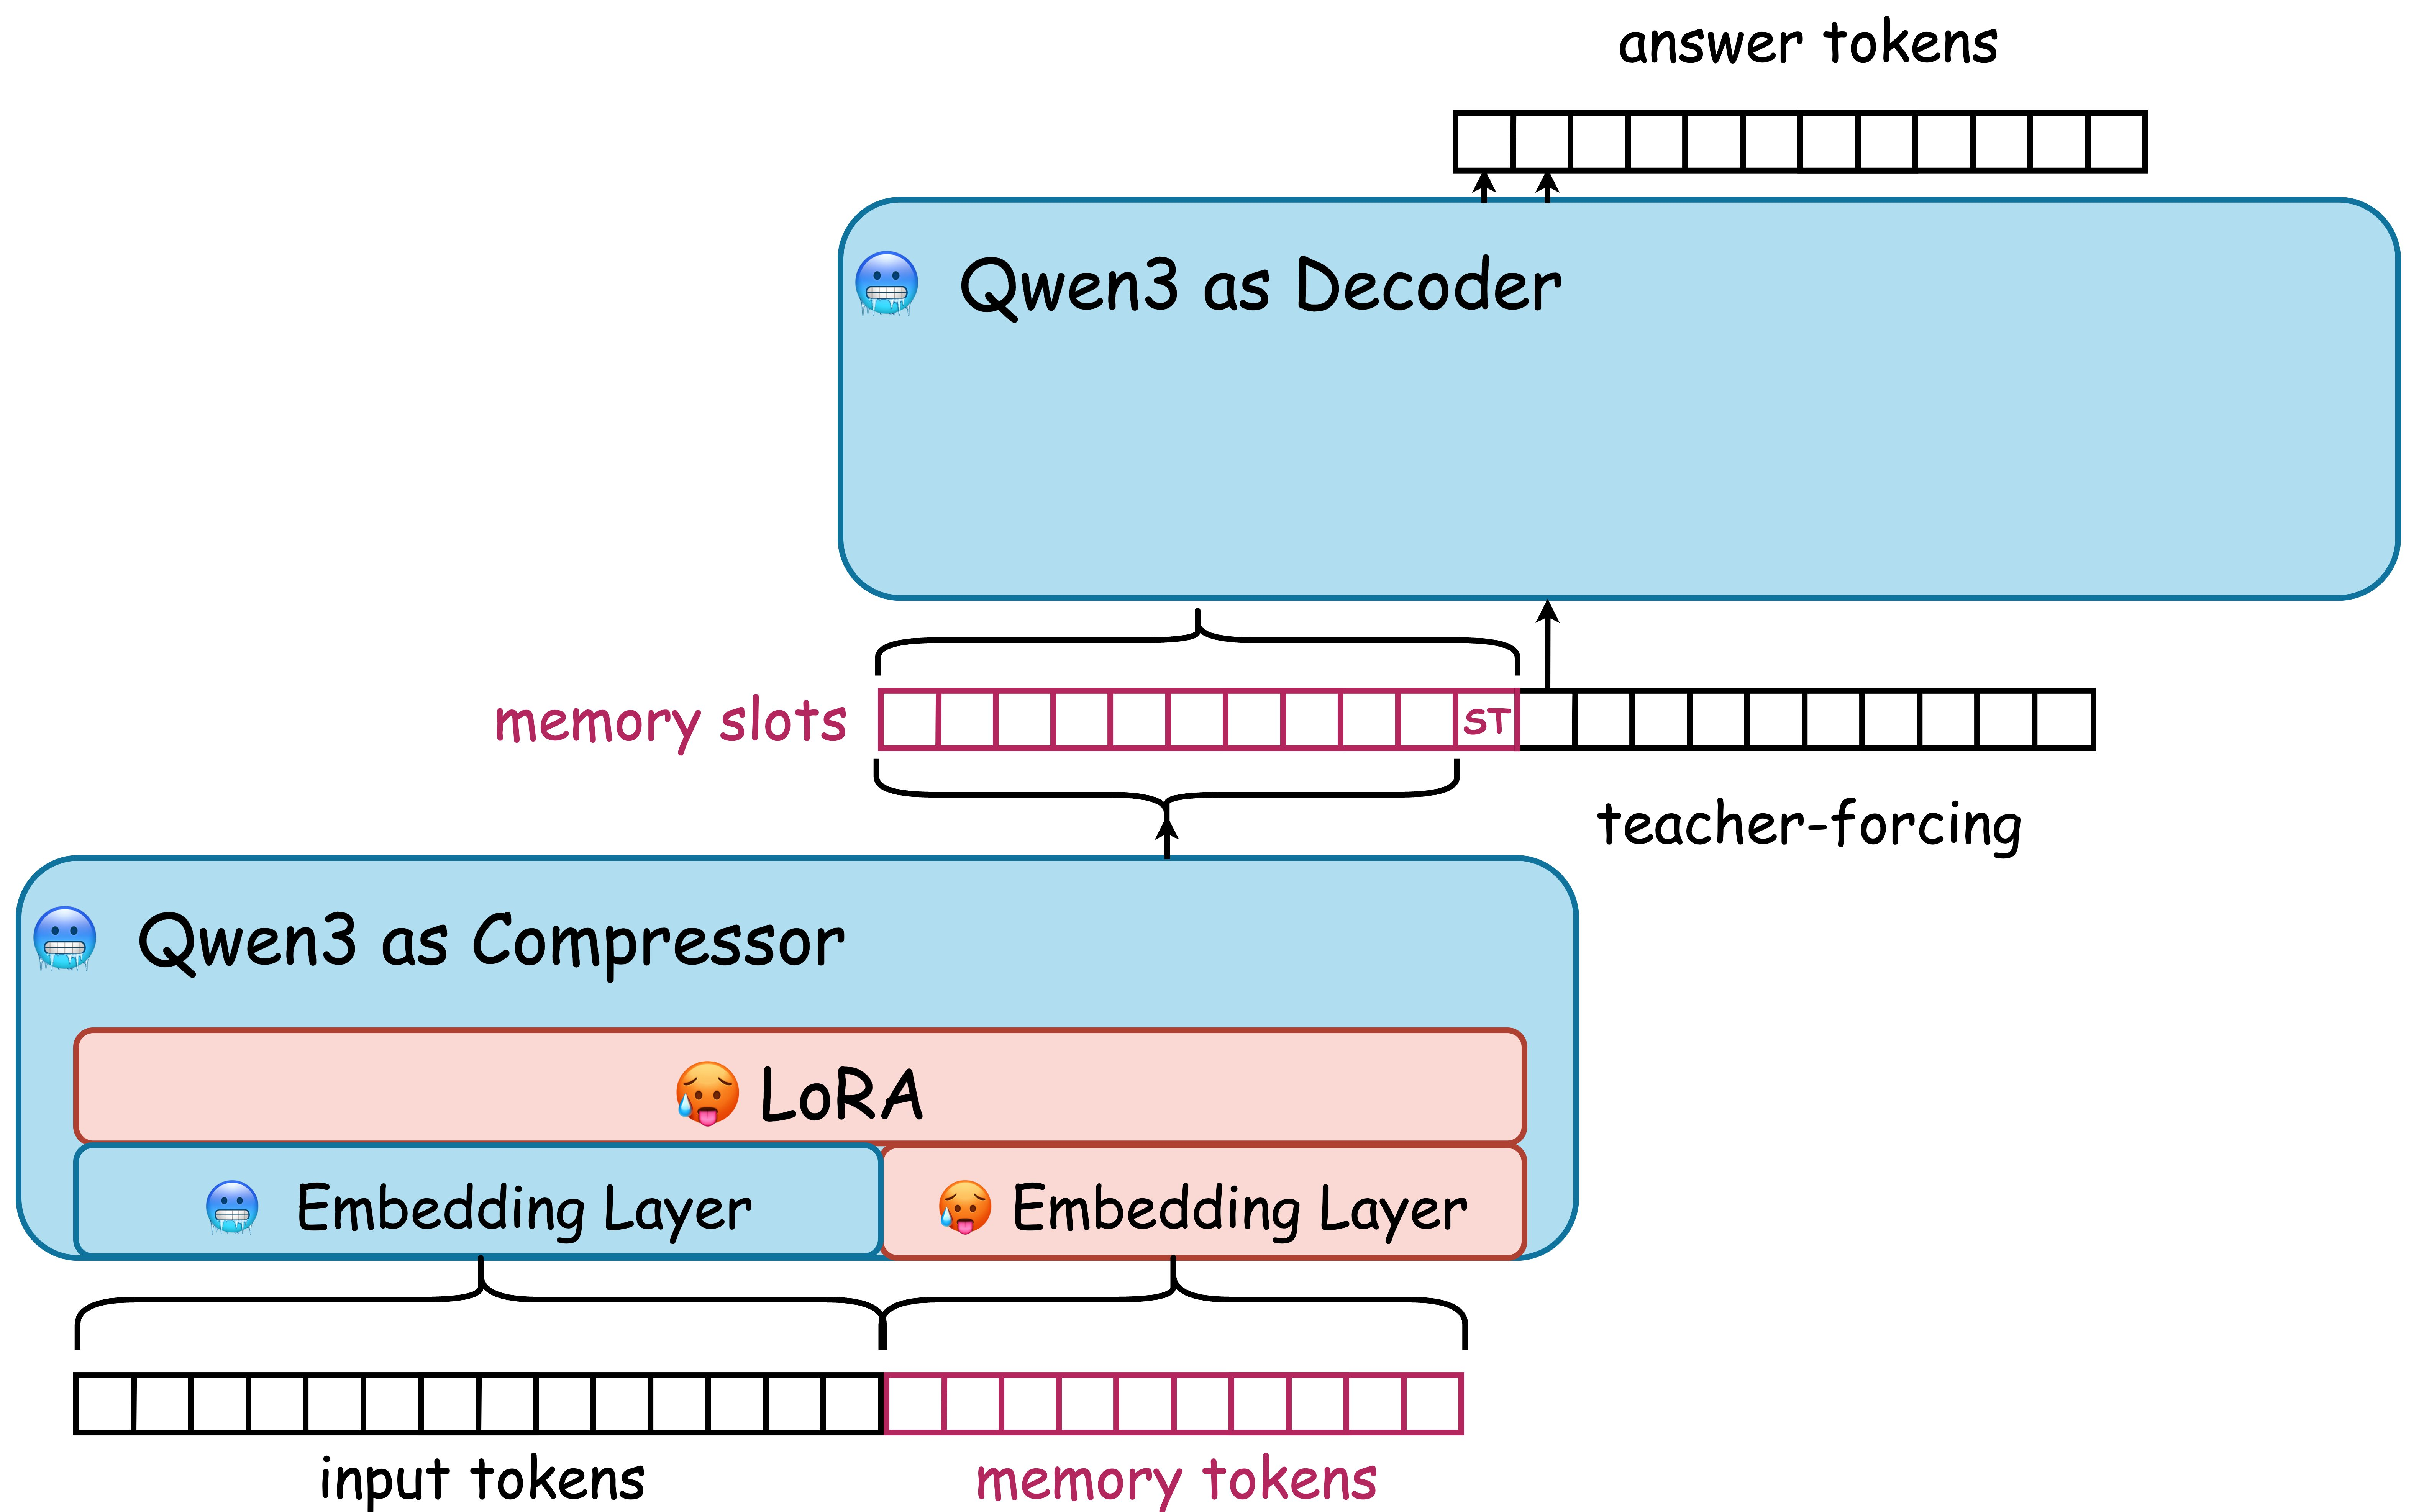
\includegraphics[width=0.8\textwidth]{graphs/icae.jpeg}
  \caption{In-Context Autoencoder (ICAE) framework architecture}
  \label{fig:icae}
\end{figure}


\section{Some attempts to do the same thing?}

Tobias' blogpost from openhands is not implicit, but explicit. so i have no knowledge of the same solutions using implicit compression?